\documentclass{article}
\usepackage{graphicx}
\usepackage{fullpage}
\usepackage{color}
\usepackage{listings}
\lstset{
basicstyle=\ttfamily,
language=C++,
%frame=single,
captionpos=b,
tabsize=2,
keywordstyle=\color{blue},
stringstyle=\color{mauve},
breaklines=true,
escapeinside={\%*}{*},
showspaces=false,
showstringspaces=false
}

\begin{document}
\title{Design of Pointer and Array Memory Objects}
\date{}
\maketitle
\section{Compositional Analysis}
\begin{figure*}[h!]
\center
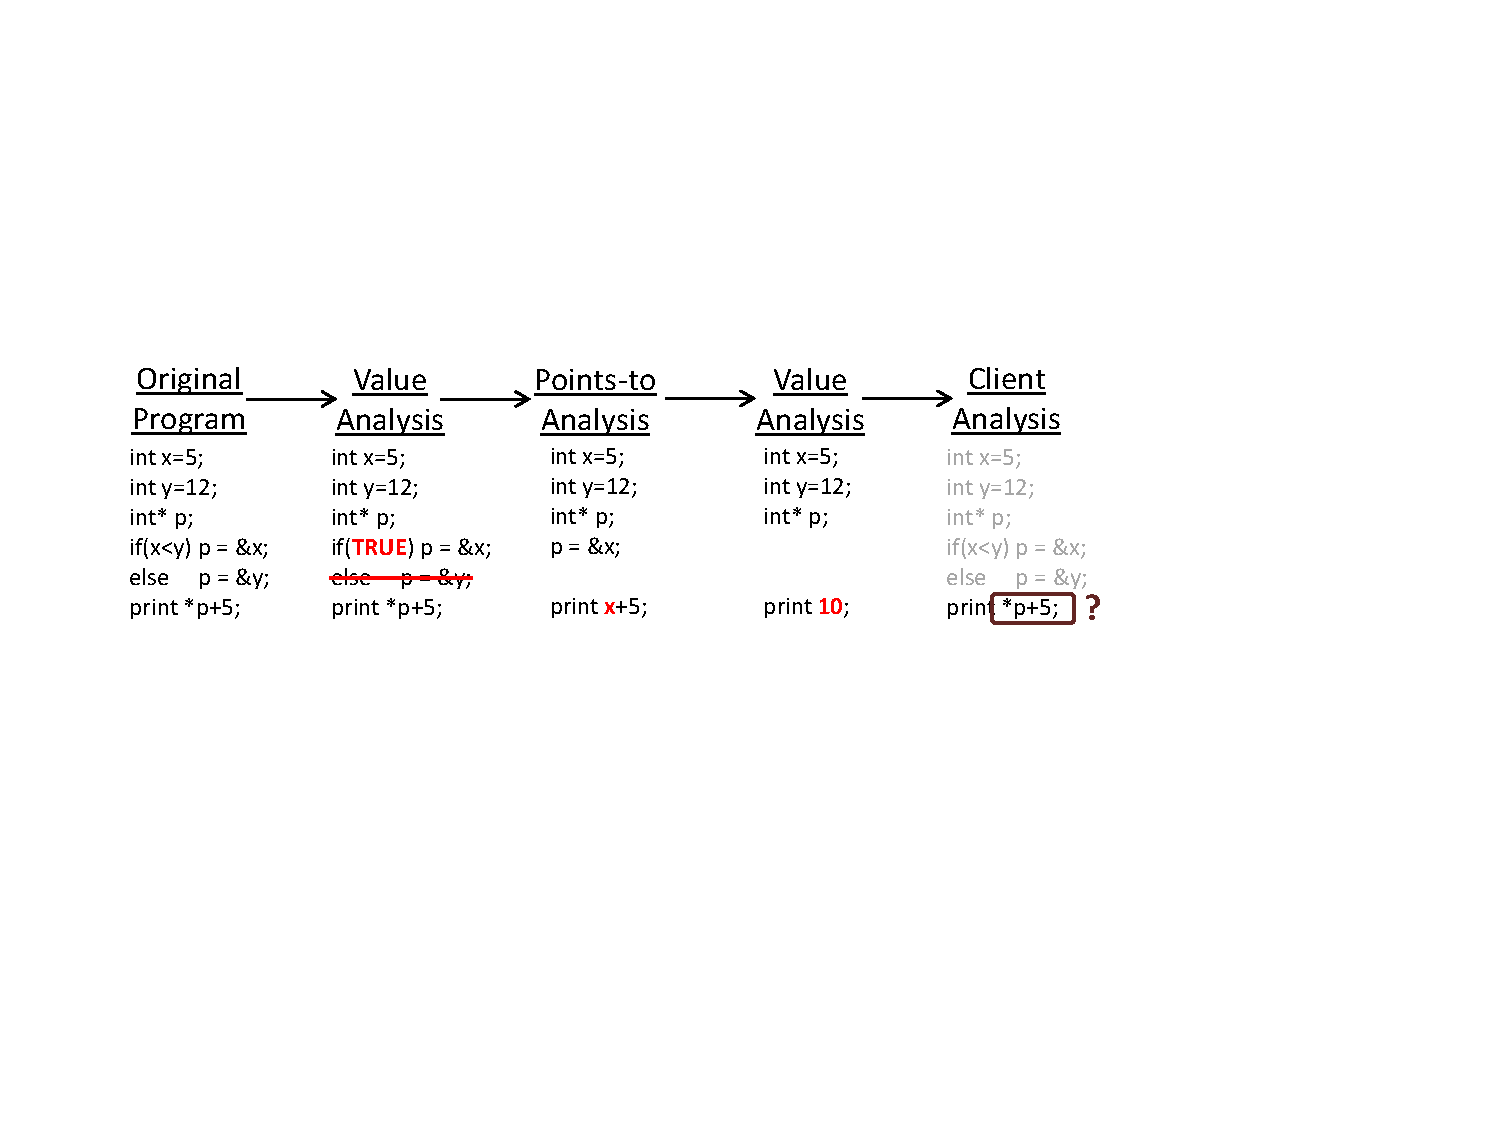
\includegraphics[width=6in]{mot_ex_chain.pdf}
\caption{Application of analysis chain to example program}
\label{fig:mot_ex_chain}
\end{figure*}

Figure~\ref{fig:mot_ex_chain} presents a simple application that requires a complex analysis account for all if its properties.
To show that it must print 10 an analysis must propagate the constant values of \texttt{x} and \texttt{y}, eliminate the dead branch of the \texttt{if} statement, propagate the points-to information from the remaining branch to the \texttt{print} operation and finally perform more constant propagation to connect the memory location of \texttt{*p} with 5 and conclude that \texttt{*p+5} is 10.
Although it is possible to perform this inference via a single integrated analysis, such monolithic analysis development is not cost-effective since it is difficult for more than a few people to contribute to the work.
As such, it is necessary to divide the overall analysis problem into multiple task-specific sub-analyses written by different people in the same or different group and somehow combine their results.
The individual analyses required to analyze this example are well known (constant propagation, dead path elimination and points-to analysis) and there exist many algorithms and implementations for these tasks.
Deployment of these analyses on real applications requires techniques to combine different types of analyses or even multiple implementations of the same analysis type into a single system.
The compositional framework allows analyses to be composed to leverage their results.



\section{Motivation}
Consider the following simple program involving pointer dereferencing expressions.
\lstset{
caption=Motivating Example,
label=code:mot-example
}
\begin{lstlisting}
void fun()
{
  int val, *p, **q;
  p = &val;
  q = &p;
  *p = 10;
  **q = **q + 1;
}
\end{lstlisting}

\noindent Inorder to correctly determine the value of \texttt{*p} and \texttt{**q} in the piece of
code in  Listing \ref{code:mot-example}, the constant propagation analysis needs to
implement the transfer function for the $=$ operator (SgAssignOp) in which
the dataflow state on rhs is transferred to the lhs. Listing  \ref{code:transfer-eq} shows a partial
implementation  of the transfer function. In general the client
(constant propagation analysis or any analysis)  requests the composer for memory
objects  corresponding to parts it may encounter in its transfer
functions. Section \ref{sec:composer} briefly discusses the interactions between client, server and composer. Similar to our example in Listing \ref{code:mot-example},
the dereferencing expression on the lhs and rhs of the $=$ operator in the last two statements can be
arbitrarily  complex, often involving arrays. We call these dereferencing expressions on lhs, rhs as dereferencing sub-expressions. 
The lhs of $=$ operator should always be a memory object corresponding to a location (see Section
\ref{sec:sem-of-eq-op}  for the semantics of the equals operator).
The default implementation  (syntax analysis) responds to the query \texttt{composer->Expr2MemLoc()} with PointerExprObj and
ArrayExprObj  for the dereferencing sub-expressions involving pointers and arrays
respectively. ExprObj are memory abstractions for temporary memory locations and they do not correspond to a particular memory location.
In this example, modifying the state for PointerExprObj on lhs as returned by syntax analysis
is incorrect  since it does not correspond to the actual memory
location. The  framework however supports getDereference() method for
Pointer/Array based objects. The semantics of the getDereference()
method is  to return the object pointed to by the corresponding
dereferencing sub-expression. The analysis writer is burdened with
interpreting  these complex dereferencing sub-expressions using only the getDereference() to
get to the valid memory object. For Array dereferencing sub-expressions, this is even difficult as it involves index.

\lstset{
label=code:transfer-eq,
caption=Transfer Function for Equals Operator
}
\begin{lstlisting}
void visit(SgAssignOp* sgn)
{
  MemLocObjectPtrPair lhsMem = composer->Expr2MemLoc(sgn->lhs_operand());
  MemLocObjectPtrPair rhsMem = composer->Expr2MemLoc(sgn->rhs_operand());
  // Get Lattices for the lhsMem, rhsMem, '=' operator
  // Copy the state from rhs to lhs and to the '=' operator
}
\end{lstlisting}

\noindent Instead of the getDereference() method, a cleaner API should
treat Pointer/Array dereferencing sub-expressions similar to variable
references and the composer/server analysis should be responsible for
returning the appropriate memory object for these expressions. The client should be completely
ignorant of the complexity of the sub-expression and merely query
the composer for the memory object of a given sub-expression. There are two options.
\begin{itemize}
\item Interpret dereferencing sub-expressions in Server Analysis (Section \ref{sec:interp-deref-exp-server})
\item Interpret dereferencing sub-expressions in Composer (Section \ref{sec:interp-deref-exp-composer})
\end{itemize}

NOTE: How should we implement \texttt{Expr2Val(**q)} on the rhs of an expression.

\section{Semantics of Equals Operator}
The $=$ operator distinguishes mutable and immutable memory regions. In C/C++ the semantics of $=$ operator is an assignment to a mutable memory region similar to the construct
\texttt{set!} in scheme and \texttt{mutable} in OCaml. In scheme, the statement \texttt{ (set! a 5)} results in the assignment of 5
the to the scalar 'a' and 'a' can be reset to any value later in code. Immutable memory  in C/C++ correspond to temporary
sub-expressions such as the value of \texttt{a+b} similar to \texttt{let} and \texttt{define} bindings in scheme. Note that 'a' or 'b' might themselves be mutable, however the temporary value of the sub-expression \texttt{a+b} is not mutable. In the current framework, we should identify all syntactically valid sub-expressions that may result in an assignment to a mutable memory region (for exampe SgVarRefExp, SgPointerDerefExp when appearing on the lhs) and the framework should make sure that it returns valid memory objects for these sub-expressions and not ExprObjects.
\label{sec:sem-of-eq-op}

\section{Composer}
\label{sec:composer}
Before discussing the interface it is important to understand the interactions between the client, server and the composer. 

\subsection{ComposedAnalysis}
Every dataflow analysis inherits ComposedAnalysis. A ComposedAnalysis may optionally implement the following functions.
\lstset{
label=code:composed-analysis-interface,
caption=Composed Analysis Interface
}
\begin{lstlisting}
ComposedAnalysis::Expr2Val()
ComposedAnalysis::OperandExpr2Val()
ComposedAnalysis::Expr2MemLoc()
ComposedAnalysis::OperandExpr2MemLoc()
ComposedAnalysis::Expr2CodeLoc()
\end{lstlisting}
These functions are useful for the analysis to export its results to the other client analysis interested in its results. Additionally each analysis maintains a pointer to the Composer.

\lstset{
label=code:composer-interface,
caption=Composer Interface
}
\subsection{Composer}
Any implementation of a Composer should imeplement the following functions.
\begin{lstlisting}
Composer::Expr2Val()
Composer::OperandExpr2Val()
Composer::Expr2MemLoc()
Composer::OperandExpr2MemLoc()
Composer::Expr2CodeLoc()
\end{lstlisting}

A client analysis in its transfer function invokes \texttt{composer->Expr2*()} or \texttt{composer->OperandExpr2*()}. Note that all analysis maintain a pointer to the Composer. The Composer maintains the list of analyses that has already finished. The composer also maintains a pointer to each analysis. In its implementation of \texttt{Composer::Expr2*()}, the composer calls \texttt{analysis->Expr2*()}. If the analysis does not have an implementation for \texttt{Expr2*()}, then an exception is thrown which is picked up the composer and the composer tries again with other analyses higher up the chain. 

\section{Interpret Dereferencing Sub-Expressions in Server Analysis}
\label{sec:interp-deref-exp-server}
This approach is intuitive and framework already supports a way to have this functionality. 
\begin{itemize}
\item Client makes the query \texttt{composer->Expr2MemLoc(sub-exp)}
\item The composer passes this query to a server analysis by calling \texttt{Expr2MemLoc} of the server analysis
\item The server analysis should handle dereferencing sub-expressions in its implementation of \texttt{Expr2MemLoc}
\item Server analysis finds the object for the given derefrencing sub-expression and returns the object to the composer which is then returned to the client.
\end{itemize}
Consider the following sequence of analyses (i) Points-to Analysis (server) (ii) Constant Propagation Analysis (client). The points-to analysis has the 
necessary information in the form of points-to graph [Fig \ref{fig:ptg-example1}] for the code in Listing \ref{code:mot-example}. With this information it is possible to infer that the expressions \texttt{*p, **q} correspond to memory object for the scalar variable \texttt{val}.
\begin{figure}[h]
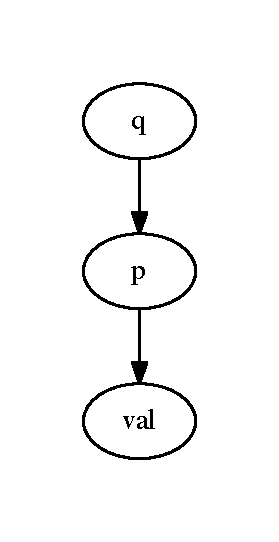
\includegraphics[scale=0.5]{ptg-example1.pdf}
\caption{Points-to Graph for Motivating Example}
\label{fig:ptg-example1}
\end{figure}

It is reasonable to expect that a points-to analysis will support dereferencing operations in its implementation of \texttt{Expr2MemLoc}. Given a query for \texttt{**q}, the points-to analysis knows that its a double dereference and it traverses the points-to graph from q twice to return the memory object corresponding to $val$. The analysis has all the necessary information to discover the memory object for arbitrary complex dereferencing sub-expressions and client has no use for the getDereference() method. In the current framework, the syntax analysis should be modified to handle pointer/array dereferencing.

\section{Interpret Dereferencing Sub-Expressions in Composer}
\label{sec:interp-deref-exp-composer}
\begin{itemize}
\item Client makes the query \texttt{composer->Expr2MemLoc(sub-exp)}
\item Instead of asking a server analysis, the composer responds with the appropriate memory object.
\item For example to interpret *p, composer calls OperandExpr2MemLoc(*p, p). This function returns the memory object corresponding to 'p' involved in the expression $*p$. Composer then invokes some API functions to access the internal data structure of the analysis inorder to answer the query.
\end{itemize}
The downside of this approach is that the a common API to access the internal data structure of analysis needs to be established. Note that the analyses can be orthogonal constraining values or memory and the API has to account for different types of analyses.

\end{document}